
\documentclass{ppgeesa}

%%%%%%%%%%%%%%%%%%%%%%%%%%%%%%%%%%%%%%%%%%%%%%%%%%%%%%%%%%%%%%%%%%%%%%%%%%%%%%%%%%%%%%%%%%%%%%%%%%%%%%%%%%%%%%%%%

\usepackage[latin1]{inputenc}
\usepackage{graphicx}
\usepackage{hyperref}
\usepackage{tikz}
\usepackage{amsmath}
\usepackage{listings}

\lstset{ %
language=Matlab,                % choose the language of the code
basicstyle=\footnotesize,       % the size of the fonts that are used for the code
numbers=none,                   % where to put the line-numbers
numberstyle=\footnotesize,      % the size of the fonts that are used for the line-numbers
stepnumber=2,                   % the step between two line-numbers. If it's 1 each line 
                                % will be numbered
numbersep=5pt,                  % how far the line-numbers are from the code
backgroundcolor=\color{white},  % choose the background color. You must add \usepackage{color}
showspaces=false,               % show spaces adding particular underscores
showstringspaces=false,         % underline spaces within strings
showtabs=false,                 % show tabs within strings adding particular underscores
frame=false,	                % adds a frame around the code
tabsize=2,		                % sets default tabsize to 2 spaces
captionpos=b,                   % sets the caption-position to bottom
breaklines=true,                % sets automatic line breaking
breakatwhitespace=true,         % sets if automatic breaks should only happen at whitespace
title=\lstname,                 % show the filename of files included with \lstinputlisting;
                                % also try caption instead of title
escapeinside={\%*}{*)}         % if you want to add a comment within your code
%morekeywords={*,...}            % if you want to add more keywords to the set
}
\lstset{caption=Descriptive Caption Text,label=DescriptiveLabel}


% reference : http://en.wikibooks.org/wiki/LaTeX/Hyperlinks
\hypersetup{
    bookmarks=true,												% show bookmarks bar?
    unicode=false,												% non-Latin characters in Acrobat�s bookmarks
    pdftoolbar=true,											% show Acrobat�s toolbar?
    pdfmenubar=true,											% show Acrobat�s menu?
    pdffitwindow=false,											% window fit to page when opened
    pdfstartview={FitH},										% fits the width of the page to the window
    pdftitle={Modelagem e identifica��o de sistemas},			% title
    pdfauthor={Tassiano Neuhaus (tassianors@gmail.com)},		% author
    pdfsubject={M�todos param�tricos de identifica��o de sistemas},   % subject of the document
    pdfcreator={Tassiano Neuhaus},								% creator of the document
    pdfproducer={Producer},										% producer of the document
    pdfkeywords={Identifica��o de sistemas} {M�todos param�tricos}, % list of keywords
    pdfnewwindow=true,											% links in new window
    colorlinks=true,											% false: boxed links; true: colored links
    linkcolor=black,											% color of internal links
    citecolor=red,												% color of links to bibliography
    filecolor=magenta,											% color of file links
    urlcolor=blue												% color of external links
}

%%%%%%%%%%%%%%%%%%%%%%%%%%%%%%%%%%%%%%%%%%%%%%%%%%%%%%%%%%%%%%%%%%%%%%%%%%%%%%%%%%%%%%%%%%%%%%%%%%%%%%%%%%%%%%%%%


\begin{document}

\title{Identifica��o de sistemas lineares - Trabalho 5}

\author{Tassiano Neuhaus\\
{\small Universidade Federal do Rio Grande do Sul - Departamento de Engenharia El�trica\\Av. Osvaldo Aranha, 103 - Bairro Bom Fim CEP: 90035-190 - Porto Alegre - RS - Brasil}\\
}%\thanks{Tassiano Neuhaus, tassianors@gmail.com, tel +55-51-91760154}}

\maketitle
\thispagestyle{empty}\pagestyle{empty}

\begin{abstract}
Identificar um modelo ARX para um processo que n�o pode ser representado por este modelo e
tamb�m um modelo completo. Ao fim, ser� feito um comparativo qualitativo das duas estimativas 
obtidas.
\end{abstract}

\begin{IEEEkeywords}
Identifica��o de sistemas lineares, m�todos param�tricos.
\end{IEEEkeywords}

%===============================================================================
\section{Introdu��o}

Neste trabalho ser� apresentado o projeto de controladores denominados Robustos. Para 
tanto ser� apresentado o conceito de um controlador Robusto. A fim de modelar um
sistema sujeito a incertezas ser� apresentado alguns m�todos para que sua modelagem
matem�tica seja poss�vel. 

Para tornar o estudo mais claro ser� utilizado um sistema f�sico onde estar� sujeito a
perturba��es e/ou incertezas. Sobre este sistema ser� feito a modelagem seguindo cada um
dos processos e com estes modelos ser� efetuado uma simula��o. 

Esta simula��o ser� baseada no projeto de uma realimenta��o de estados com o intuito de
satisfazer a minimiza��o da norma $H2$ e $H_{\infty}$.

O sistema utilizado � apresentado no sistema de equa��es de estado descrito em (\ref{eq:intro_sis}).

\begin{equation}
\begin{matrix}
A=\begin{bmatrix}
0 & 1\\ 
-ba &a+b 
\end{bmatrix} &
B=\begin{bmatrix}
0\\ 
k
\end{bmatrix} 
\end{matrix}
\label{eq:intro_sis}
\end{equation}

Este sistema possui a fun��o de transfer�ncia apresentado em (\ref{eq:intro_transf}).

\begin{equation}
G(s)=\frac{k}{(s-a)(s-b)}
\label{eq:intro_transf}
\end{equation}

Os par�metros $a, b, k$ est�o sujeitos as varia��es apresentadas em (\ref{eq:intro_limit}).

\begin{equation}
\begin{matrix}
b= & -0.012725 & \\ 
k= & [k_1 \; k_2] =& [-0.4649.10^{-4} \; -0.7449.10^{-4}]\\ 
a= & [a_1 \; a_2] =& [-0.25 \; -2]
\end{matrix}
\label{eq:intro_limit}
\end{equation}


\section{Modelo ARX}
\label{sec:arx}
%===============================================================================

O sistema real apresentado em (\ref{eq:system}) ser� identificado pelo modelo ARX onde
genericamente o modelo utilizado � como apresentado em (\ref{eq:generic_model}) e 
para o modelo ARX tem-se que apenas os polin�mios $A$ e $B$ s�o diferentes de 1. \cite{aguirre}

\begin{equation}
A(q, \theta)Y(t)=\frac{B(q, \theta)}{F(q, \theta)}U(t)+\frac{C(q, \theta)}{D(q, \theta)}e(t)
\label{eq:generic_model}
\end{equation}

Onde:

\begin{equation}
\begin{matrix}
A(q, \theta)=1+a_1 q^{-1}+a_2 q^{-2}+\cdots +a_{na} q^{-na}\\
B(q, \theta)=b_1 q^{-1}+b_2 q^{-2}+\cdots +b_{nb} q^{-nb}\\ 
C(q, \theta)=1+c_1 q^{-1}+c_2 q^{-2}+\cdots +c_{nc} q^{-nc}\\ 
D(q, \theta)=1+d_1 q^{-1}+d_2 q^{-2}+\cdots +d_{na} q^{-nd}\\ 
F(q, \theta)=1+f_1 q^{-1}+f_2 q^{-2}+\cdots +f_{nf} q^{-nf} 
\end{matrix}
\nonumber
\end{equation}

Desta forma o modelo ARX pode ser representado como em (\ref{eq:model_arg_g}). Para o
sistema apresentado em (\ref{eq:system}), o modelo ARX fica como em (\ref{eq:model_arx}).

\begin{equation}
A(q, \theta)Y(t)=B(q, \theta)U(t)+e(t)
\label{eq:model_arx_g}
\end{equation}

\begin{equation}
G(q, \theta )=\frac{a}{q-b}\;\;\;\;\;H(q, \theta)=\frac{q}{q-b}
\label{eq:model_arx}
\end{equation}

\begin{equation}
y(t)=G(q, \theta)r(t)+H(q, \theta)e(t)
\nonumber
\end{equation}

Onde $e(t)$ � ruido branco com m�dia zero.

Este modelo n�o consegue representar o sistema descrito em (\ref{eq:system}). 
Foi utilizado o script do matlab apresentado no Anexo (\ref{anx_arx_simul}) para 
simular as estimativas obtidas para os par�metros $a$ e $b$ deste modelo, o script
utiliza o m�todo dos m�nimos quadrados para estimar os par�metros.

O resultado da simula��o � apresentado na Figura (\ref{fig:arx}).

\begin{figure}[htbp]
	\center
	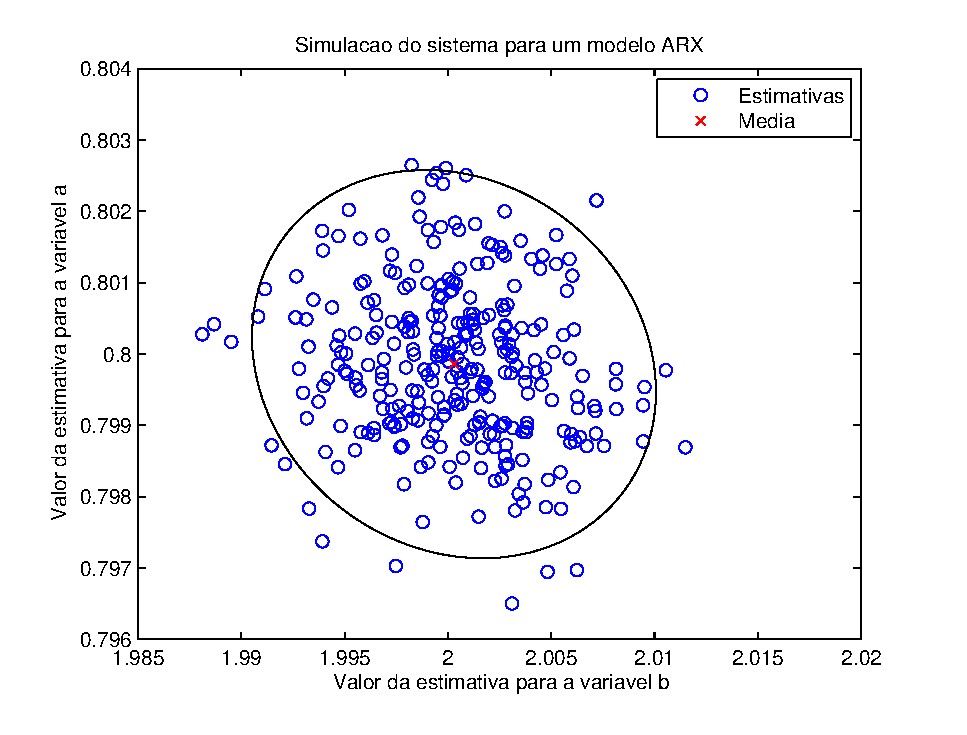
\includegraphics[width=0.98\columnwidth]{figures/arx.eps}
	\caption{Simula��o do sistema para uma entrada aleat�ria e utilizando o modelo ARX.}
	\label{fig:arx}
\end{figure}

A m�dia das estimativas obtidas para o sistema foi de $a=2.003$ e $b=0.7999$.

Aplicando na entrada do processo uma senoide de frequ�ncia $\pi /4$ obt�m-se a estimativa
como apresentado na Figura (\ref{fig:arx_sin_pi4}).

\begin{figure}[htbp]
	\center
	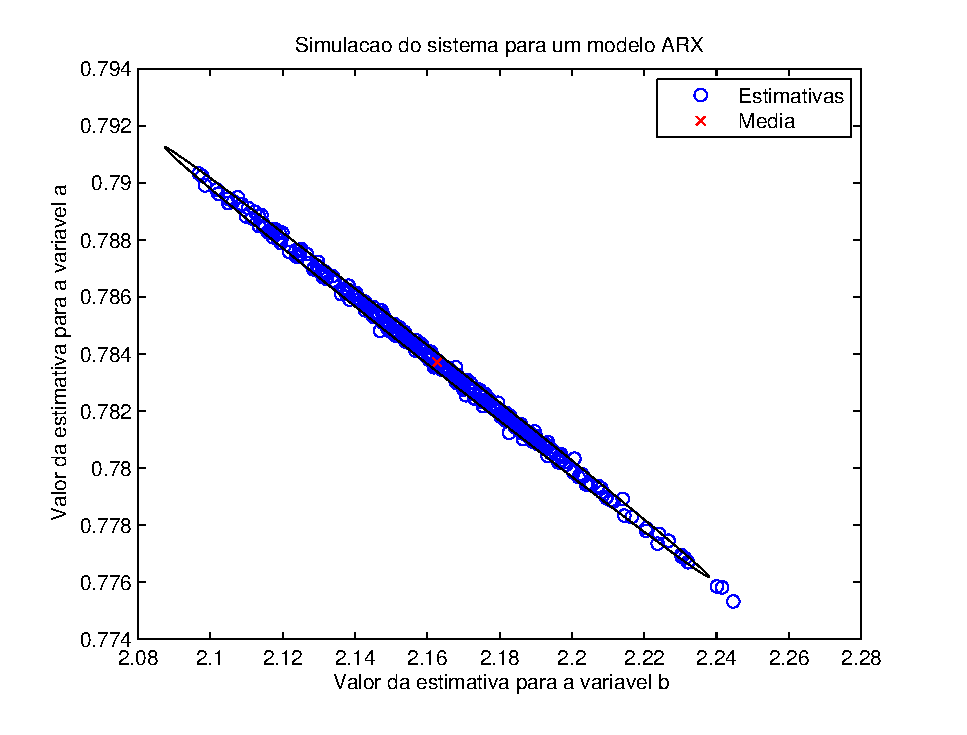
\includegraphics[width=0.98\columnwidth]{figures/arx_sin_pi4.eps}
	\caption{Simula��o do sistema para uma entrada $sin(\pi /4)$ e utilizando o modelo ARX.}
	\label{fig:arx_sin_pi4}
\end{figure}

A m�dia das estimativas obtidas para o sistema foi de $a=2.1627$ e $b=0.7837$.


Aplicando na entrada do processo uma senoide de frequ�ncia $\pi /20$ obt�m-se a estimativa
como apresentado na Figura (\ref{fig:arx_sin_pi20}).

\begin{figure}[htbp]
	\center
	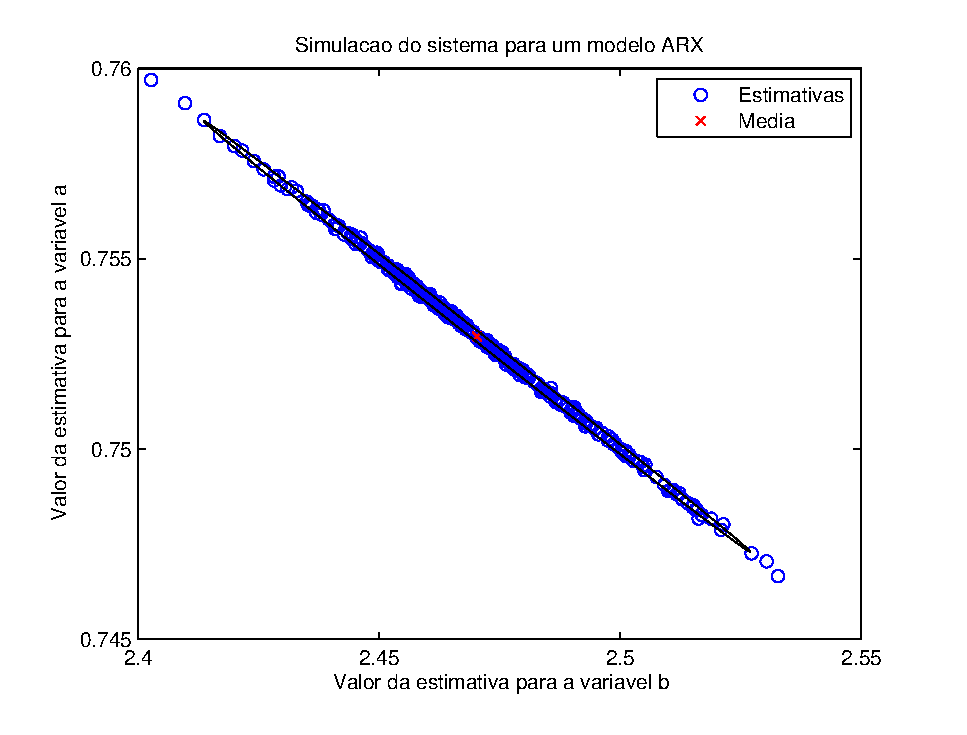
\includegraphics[width=0.98\columnwidth]{figures/arx_sin_pi20.eps}
	\caption{Simula��o do sistema para uma entrada $sin(\pi /4)$ e utilizando o modelo ARX.}
	\label{fig:arx_sin_pi20}
\end{figure}

A m�dia das estimativas obtidas para o sistema foi de $a=2.1687$ e $b=0.7831$.

Observa-se claramente que a estimativa est� polarizada, ou seja, a m�dia das estimativas 
n�o est� centrada nos valores reais dos par�metros. Isso de deve ao fato que o modelo utilizado
para a estimativa n�o consegue representar na totalidade o sistema original.


\section{Modelo Completo}
\label{sec:non_arx}
%===============================================================================

Como apresentado na sec�o (\ref{sec:arx}) o modelo ARX n�o consegue representar o
sistema (\ref{eq:system}) completamente, e a estimativa dos parametros da Func�o
de transferencia s�o polarizados. Para contornar este problema utilizaremos um
modelo para descrever o sistema (\ref{eq:system}) de forma completa.

O modelo escolhido para representar o sistema real � apresentado em (\ref{eq:compl}).

\begin{equation}
G(q, \theta )=\frac{a}{q-b}\;\;\;\;\;H(q, \theta)=\frac{q-c}{q-d}
\label{eq:compl}
\end{equation}



%===============================================================================
\section{Conclus�es}
\label{sec:concl}
%===============================================================================

Neste trabalho foram apresentados dois m�todos para identifica��o de sistemas lineares,
ambos os m�todos se encontram na categoria de m�todos param�tricos de identifica��o, que 
de forma simplificada, tentam estimar os par�metros de uma fun��o de transfer�ncia que
represente o sistema f�sico em quest�o. Os m�todos utilizados foram o dos m�nimos quadrados
e das vari�veis instrumentais.

O sistema f�sico utilizado foi o controle de posi��o de um motor DC, e os dados coletados
para a identifica��o foram gerados a partir da aplica��o de sinais de refer�ncia tais como
rampas, senoides e ondas quadradas. Para cada um destes conjuntos foi obtido uma estimativa
dos par�metros do modelo utilizado.

Para efetuar a estimativa do sistema f�sico em quest�o, foi necess�rio determinar um modelo,
este foi determinado baseado no conhecimento das caracter�sticas do sistema e algumas simplifica��es 
foram efetuadas, a fim de tornar o modelo matem�tico o mais simples poss�vel, mas que ainda 
consiga descrever o sistema dentro de uma margem aceit�vel de precis�o.

O m�todo dos m�nimos quadrados (\ref{sec:mmq}) obteve resultados para a estimativa dos par�metros
que podem ser encontrados na Tabela (\ref{tab:mmq_results}). Houveram pequenas diverg�ncias nos 
par�metros entre um conjunto de dados e outro, o que n�o � desej�vel, isso pode ser devido a
imprecis�es do modelo utilizado, (pode ser devido as simplifica��es do modelo, ou de din�micas n�o
levadas em considera��o).

O m�todo das vari�veis instrumentais (\ref{sec:iv}) obteve resultados semelhantes ao m�todo 
dos m�nimos quadrados, mas com valores mais pr�ximos nos diferentes grupos de medidas. Os 
resultados para este m�todo foram apresentados na Tabela (\ref{tab:iv_results}).

De forma geral este trabalho abordou e demonstrou como � o procedimento e no que se baseiam 
dois m�todos de identifica��o de sistemas lineares sujeitos a incertezas, perturba��es e 
ru�dos. N�o � o objetivo deste trabalho detalhar esmiu�ar a matem�tica destes m�todos e
sim apresentar um exemplo pr�tico, e demonstrar sua utilidade.

A aplicabilidade deste t�pico de engenharia � de uma aplicabilidade imensa, sendo muito importante 
nas mais diversas �reas a correta identifica��o de sistemas para que, a partir do conhecimento 
matem�tico de sua din�mica, possa se agir sobre este sistema, a fim de obter os resultados desejados
de forma eficiente e com propriedade sobre as a��es tomadas, uma vez que o sistema identificado
� identificado e sabe-se o qu�o boa esta aproxima��o do sistema real pode ser.

%===============================================================================
\appendix
%===============================================================================
\chapter{1 - Script para Simula��o do MQ para o modelo ARX} 
\label{appendix_mmq}
\lstset{caption=M�todo dos m�nimos quadrados,label=DescriptiveLabel}
\lstinputlisting{matlab_files/simul.m}

%===============================================================================
\chapter{2 - Script para Simula��o do m�todo das vari�veis instrumentais} 
\label{appendix_iv}
\lstset{caption=M�todo das vari�veis instrumentais,label=DescriptiveLabel}
\lstinputlisting{matlab_files/simul_iv.m}

%===============================================================================



\bibliographystyle{IEEEtran}
\bibliography{biblio}

\end{document}
